\documentclass[12pt, titlepage]{article}
\usepackage{graphicx}
\usepackage{booktabs}
\usepackage{tabularx}
\usepackage{float}
\usepackage{hyperref}
\hypersetup{
    colorlinks,
    citecolor=black,
    filecolor=black,
    linkcolor=red,
    urlcolor=blue
}
\usepackage[round]{natbib}

\usepackage{color}

\newif\ifcomments\commentstrue

\ifcomments
\newcommand{\authornote}[3]{\textcolor{#1}{[#3 ---#2]}}
\newcommand{\todo}[1]{\textcolor{red}{[TODO: #1]}}
\else
\newcommand{\authornote}[3]{}
\newcommand{\todo}[1]{}
\fi

\newcommand{\wss}[1]{\authornote{blue}{SS}{#1}} 
\newcommand{\plt}[1]{\authornote{magenta}{TPLT}{#1}} %For explanation of the template
\newcommand{\an}[1]{\authornote{cyan}{Author}{#1}}


\begin{document}

\title{Test Report: Stoichiometry Mass-Mass Program} 
\author{Deemah Alomair}
\date{\today}
	
\maketitle

\pagenumbering{roman}

\section{Revision History}

\begin{tabularx}{\textwidth}{p{3cm}p{2cm}X}
\toprule {\bf Date} & {\bf Version} & {\bf Notes}\\
\midrule
26/12/2019 & 1.0 & First version of the document\\
\bottomrule
\end{tabularx}

~\newpage

\section{Symbols, Abbreviations and Acronyms}

\renewcommand{\arraystretch}{1.2}
\begin{tabular}{l l} 
  \toprule		
  \textbf{symbol} & \textbf{description}\\
  \midrule 
  T & Test\\
SMMP & Stoichiometry Mass-Mass Program\\
  \bottomrule
\end{tabular}\\


\newpage

\tableofcontents

\listoftables %if appropriate

\listoffigures %if appropriate

\newpage

\pagenumbering{arabic}

This document report result from system test cases found in System Verification and Validation Plan document \cite{SystemVnVPlan}.

\section{Functional Requirements Evaluation}

Functional requirements are evaluated using system test cases from id1 to id10. All the details regarding functional requirements evaluation can be found in section ~\ref{unit}. The traceability between system test cases and functional requirements found in table ~\ref{Table:R_trace} of section ~\ref{functional}.

\section{Nonfunctional Requirements Evaluation}

Nonfunctional Requirements evaluated in system test cases id11 - id12. All the details regarding Nonfunctional requirements evaluation can be found in this section. The traceability between system test cases and Nonfunctional requirements found in table ~\ref{Table:R_trace1} of section ~\ref{functional}.


\subsection{Usability}

system test id11 measures the Usability of SMMP system. The survey measured the satisfaction level of potential user after using SMMP. How easy and understandable the system is?. It needs to be filled by any user and if satisfactory level is low then enhancement need to be taken into account. survey can be found in Appendix of  \cite{SystemVnVPlan}.
		
\subsection{Reliability}

system test id12 measures the Reliability of SMMP system. 25 different unbalanced chemical reactions were tested and compared to answer of online balancer  \cite{OnlineBalancer} as parallel testing. the aim was to get 100\% of correct answers that includes right balance reaction and correct mass value. Below table shows the final result compared to the online balancer and the final percentage of correctness.
The goal of Reliability had been accomplished. all tested reactions were balanced correctly as compared to the online balancer.

\begin{table}[h!]
\centering
\resizebox{\textwidth}{!}{\begin{tabular}{|c|c|c|c|}
\hline
 Unbalanced Chemical Reaction & Online Balancer Result & SMMP Result  & correctness \\
\hline
C$H_4$ + $O_2$ $\rightarrow$ C$O_2$ + $H_2$O  & C$H_4$ + 2$O_2$ $\rightarrow$ C$O_2$ + 2$H_2$O  & C$H_4$ + 2$O_2$ $\rightarrow$ C$O_2$ + 2$H_2$O  &  correct  \\ \hline
$Fe_2$$O_3$ + C $\rightarrow$ Fe + C$O_2$  & 2$Fe_2$$O_3$ + 3C $\rightarrow$ 4Fe + 3C$O_2$ & 2$Fe_2$$O_3$ + 3C $\rightarrow$ 4Fe + 3C$O_2$ & correct   \\ \hline
$N_2$ + $O_2$ $\rightarrow$ $N_2$$O_5$ & 2$N_2$ + 5$O_2$ $\rightarrow$ 2$N_2$$O_5$ & 2$N_2$ + 5$O_2$ $\rightarrow$ 2$N_2$$O_5$& correct  \\ \hline
C$H_4$ + $Cl_2$ $\rightarrow$  C$Cl_4$ + HCl & C$H_4$ + 4$Cl_2$ $\rightarrow$  C$Cl_4$ + 4HCl & 4C$H_4$ + $Cl_2$ $\rightarrow$  C$Cl_4$ + 4HCl & correct   \\ \hline
$N_2$ + $H_2$ $\rightarrow$ $NH_3$ & $N_2$ + 3$H_2$ $\rightarrow$ 2$NH_3$ & $N_2$ + 3$H_2$ $\rightarrow$ 2$NH_3$ & correct \\ \hline
Fe + $H_2$O $\rightarrow$ $Fe_3$$O_4$ + $H_2$ & 3Fe + 4$H_2$O $\rightarrow$ $Fe_3$$O_4$ + 4$H_2$ & 3Fe + 4$H_2$O $\rightarrow$ $Fe_3$$O_4$ + 4$H_2$ & correct \\ \hline
Xe + $F_2$ $\rightarrow$ Xe$F_6$ & Xe + 3$F_2$ $\rightarrow$ Xe$F_6$ & Xe + 3$F_2$ $\rightarrow$ Xe$F_6$ & correct  \\ \hline
Hg + $O_2$ $\rightarrow$ HgO & 2Hg + $O_2$ $\rightarrow$ 2HgO & 2Hg + $O_2$ $\rightarrow$ 2HgO & correct  \\ \hline
CaO + C $\rightarrow$ Ca$C_2$ + CO & CaO + 3C $\rightarrow$ Ca$C_2$ + CO & CaO + 3C $\rightarrow$ Ca$C_2$ + CO & correct  \\ \hline
$S_8$ + $F_2$ $\rightarrow$ $SF_6$ & $S_8$ + 24$F_2$ $\rightarrow$ 8$SF_6$ & $S_8$ + 24$F_2$ $\rightarrow$ 8$SF_6$ & correct  \\ \hline
Mg + $N_2$ $\rightarrow$ $Mg_3$$N_2$ & 3Mg + $N_2$ $\rightarrow$ $Mg_3$$N_2$ & 3Mg + $N_2$ $\rightarrow$ $Mg_3$$N_2$ & correct  \\ \hline
Be$F_2$ + Mg $\rightarrow$ Mg$F_2$ + Be & balance & balance & correct  \\ \hline
Zn + HCl $\rightarrow$ Zn$Cl_2$ + $H_2$ & Zn + 2HCl $\rightarrow$ Zn$Cl_2$ + $H_2$ & Zn + 2HCl $\rightarrow$ Zn$Cl_2$ + $H_2$ & correct  \\ \hline
SiC + $Cl_2$ $\rightarrow$ Si$Cl_4$ + C & SiC + 2$Cl_2$ $\rightarrow$ Si$Cl_4$ + C & SiC + 2$Cl_2$ $\rightarrow$ Si$Cl_4$ + C & correct \\ \hline
MnS + HCl $\rightarrow$ $H_2$S + Mn$Cl_2$ & MnS + 2HCl $\rightarrow$ $H_2$S + Mn$Cl_2$ & MnS + 2HCl $\rightarrow$ $H_2$S + Mn$Cl_2$ & correct  \\ \hline
 U$F_4$ + Mg $\rightarrow$ Mg$F_2$ + U & U$F_4$ + 2Mg $\rightarrow$ 2Mg$F_2$ + U &  U$F_4$ + 2Mg $\rightarrow$ 2Mg$F_2$ + U & correct  \\ \hline
S + $N_2$O $\rightarrow$ S$O_2$ + $N_2$ & S + 2$N_2$O $\rightarrow$ S$O_2$ + 2$N_2$ & S + 2$N_2$O $\rightarrow$ S$O_2$ + 2$N_2$ & correct  \\ \hline
Si$H_4$ + $O_2$ $\rightarrow$ Si$O_2$ + $H_2$O & Si$H_4$ + 2$O_2$ $\rightarrow$ Si$O_2$ + 2$H_2$O & Si$H_4$ + 2$O_2$ $\rightarrow$ Si$O_2$ + 2$H_2$O & correct  \\ \hline
Ti$Cl_4$ + Mg $\rightarrow$ Mg$Cl_2$ + Ti & Ti$Cl_4$ + 2Mg $\rightarrow$ 2Mg$Cl_2$ + Ti  & Ti$Cl_4$ + 2Mg $\rightarrow$ 2Mg$Cl_2$ + Ti & correct  \\ \hline
Si + $S_8$ $\rightarrow$ $Si_2$$S_4$ & 4Si + $S_8$ $\rightarrow$ 2$Si_2$$S_4$ & 4Si + $S_8$ $\rightarrow$ 2$Si_2$$S_4$ & correct \\ \hline
Si$O_2$ + HF $\rightarrow$ Si$F_4$ + $H_2$O & Si$O_2$ + 4HF $\rightarrow$ Si$F_4$ + 2$H_2$O & Si$O_2$ + 4HF $\rightarrow$ Si$F_4$ + 2$H_2$O & correct \\ \hline
$P_4$ + $O_2$ $\rightarrow$ $P_2$$O_5$ & $P_4$ + 5$O_2$ $\rightarrow$ 2$P_2$$O_5$ & $P_4$ + 5$O_2$ $\rightarrow$ 2$P_2$$O_5$& correct \\ \hline
Sb + $O_2$ $\rightarrow$ $Sb_4$$O_6$ & 4Sb + 3$O_2$ $\rightarrow$ $Sb_4$$O_6$ & 4Sb + 3$O_2$ $\rightarrow$ $Sb_4$$O_6$ & correct \\ \hline
U$O_2$ + HF $\rightarrow$ U$F_4$ + $H_2$O  & U$O_2$ + 4HF $\rightarrow$ U$F_4$ + 2$H_2$O  & U$O_2$ + 4HF $\rightarrow$ U$F_4$ + 2$H_2$O & correct \\ \hline
Al + $O_2$ $\rightarrow$ $Al_2$$O_3$ & 4Al + 3$O_2$ $\rightarrow$ 2$Al_2$$O_3$ & 4Al + 3$O_2$ $\rightarrow$ 2$Al_2$$O_3$ & correct  \\ \hline
\hline
\end{tabular}}
\caption{Reliability testing of SMMP as comparison to online balancer.}
\label{Reliability}
\end{table}
	
\section{Comparison to Existing Implementation}	

This is stand alone system. If there is any existing systems with same functionalities and goals the developer is not aware about them and no comparison had been made.

\section{Unit Testing}\label{unit}

\subsection{Mass Input Test-id1}

The goal of this test is to make sure user enter a positive number in mass value widget. the default mass value is 1. pictures below illustrate all possible entries by user that cause error massage which matches cases of id1 ,Table1 in \cite{SystemVnVPlan}. The tests had been passed correctly and system responded as intended. 

 \begin{figure}[H]
 \begin{center}
 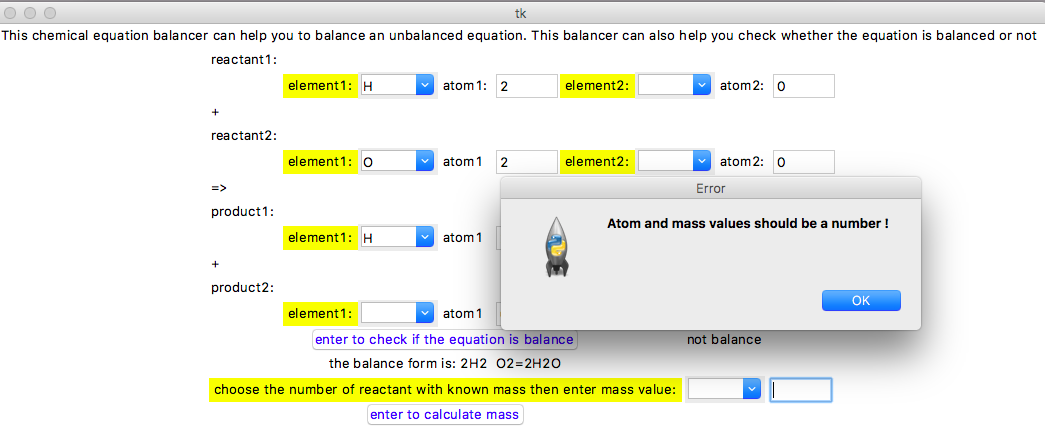
\includegraphics [width=\textwidth]{massnotnumber}
 \caption{\label{ Figure 1:} error massage if user enter non number mass value}
 \end{center}
 \end{figure}
 
\begin{figure}[H]
 \begin{center}
 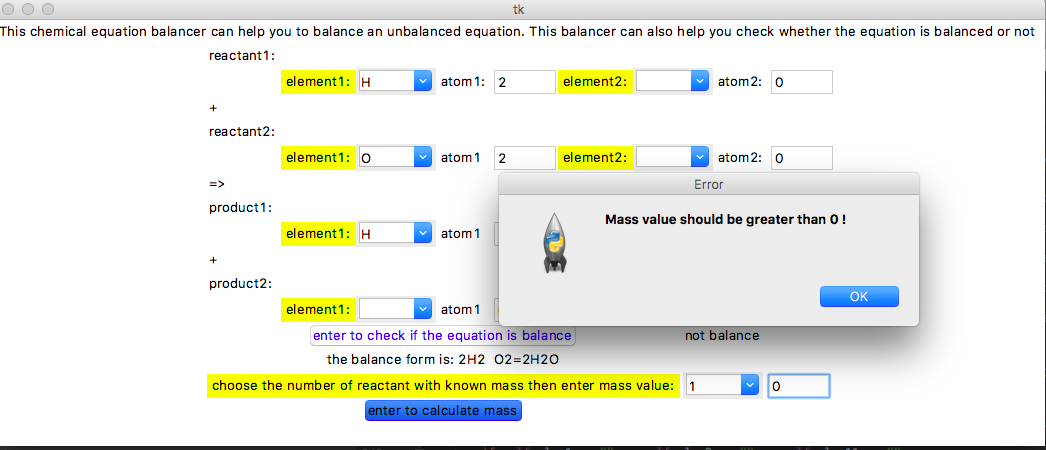
\includegraphics [width=\textwidth]{massnegative}
 \caption{\label{ Figure 2:} error massage if user enter mass less than 1}
 \end{center}
 \end{figure}

\subsection{Reaction Input Test-id2}
The goal of this test is to ensure that user had entered a correct chemical reaction format that satisfies the system requirements and enter a positive number for atom value. More details of accepted reaction format can be found in Unit Verification and Validation Plan \cite{UnitVnVPlan}  and Unit Verification and Validation Test Report \cite{VnVReport}. Test case id2 testing entered atom value. pictures bellow show all possible entires of atom value and system responds to each case. The test passed with right system behavior. 

\begin{figure}[h!]
 \begin{center}
 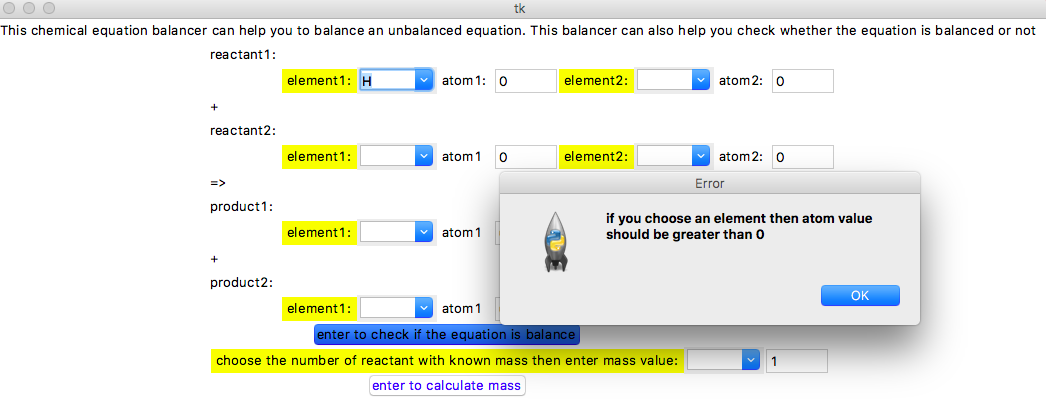
\includegraphics [width=\textwidth]{atomnegative}
 \caption{\label{ Figure 3:} error massage if user enter atom less than 1 after selecting an element}
 \end{center}
 \end{figure}
 
 \begin{figure}[h!]
 \begin{center}
 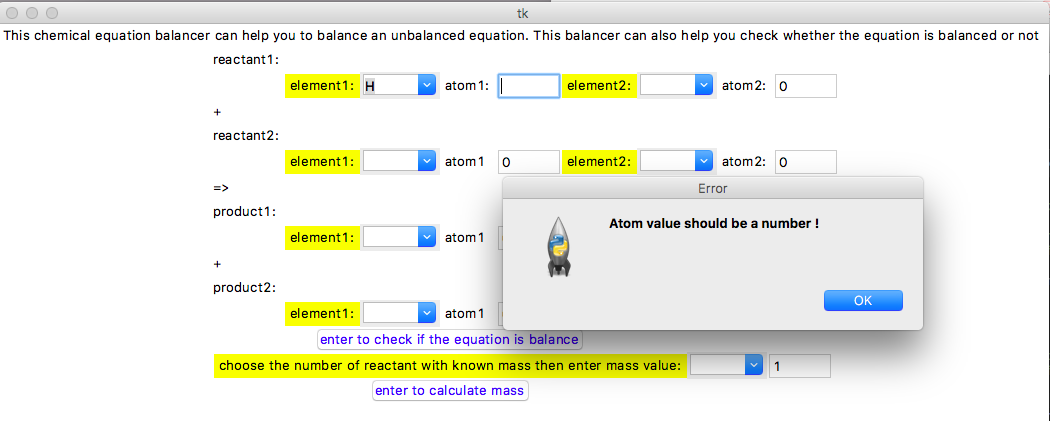
\includegraphics [width=\textwidth]{atomnotnumber}
 \caption{\label{ Figure 4:} error massage if user enter non number atom value}
 \end{center}
 \end{figure}

\subsection{Reaction Output Test-id3 , Mass Output Test-id4}

The goal of this test is to output the final result including the mass and balance reaction to GUI. This is the main goal of the system. Picture below shows how system will print out the final result to end user. This test is for test cases  id3, id4 in \cite{SystemVnVPlan}. Test passed correctly and system responded as intended.

\begin{figure}[h!]
 \begin{center}
 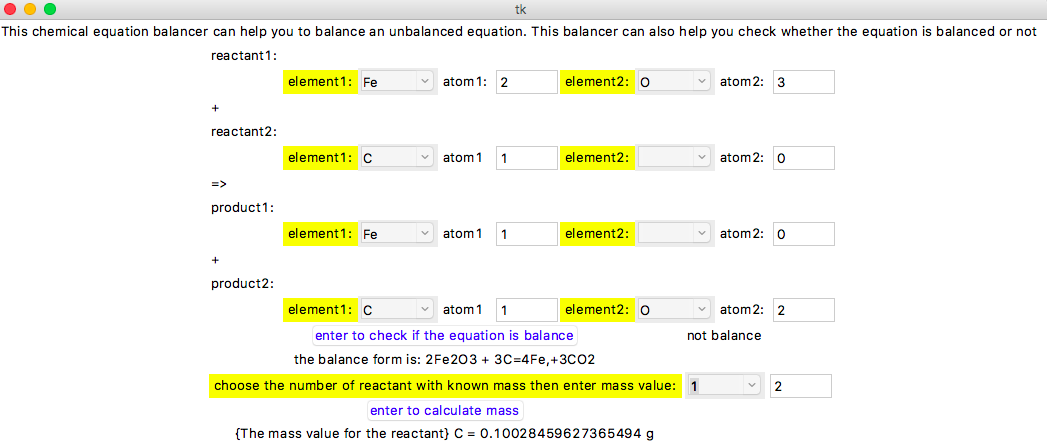
\includegraphics [width=\textwidth]{output}
 \caption{\label{ Figure 5:} final system output}
 \end{center}
 \end{figure}

\subsection{Check Balance Test-id5}

The goal of this test is to check if the entered reaction is balance or not. Display "balance" if yes and "not balance" with new balanced form if not. Pictures below show how system respond to balance and non balance reactions. The test passed correctly and system responded as intended.

\begin{figure}[H]
 \begin{center}
 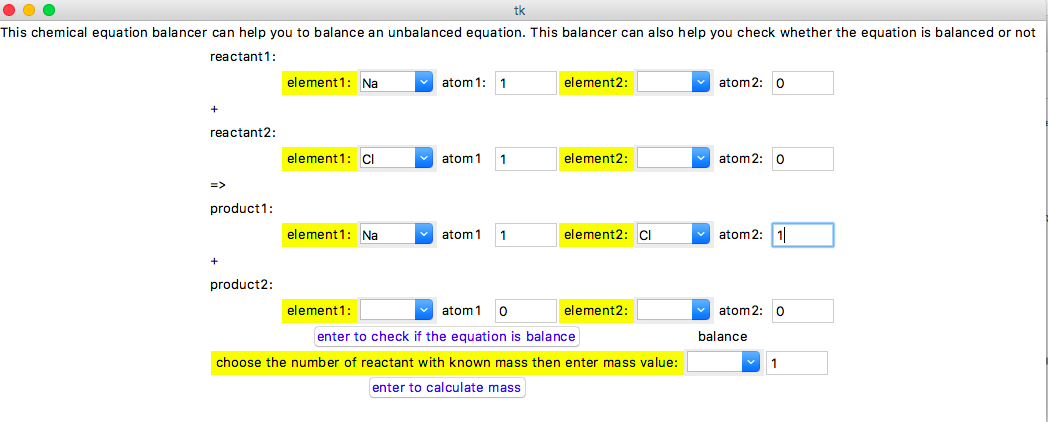
\includegraphics [width=\textwidth]{balance}
 \caption{\label{ Figure 6:} balance reaction}
 \end{center}
 \end{figure}
 
\begin{figure}[H]
 \begin{center}
 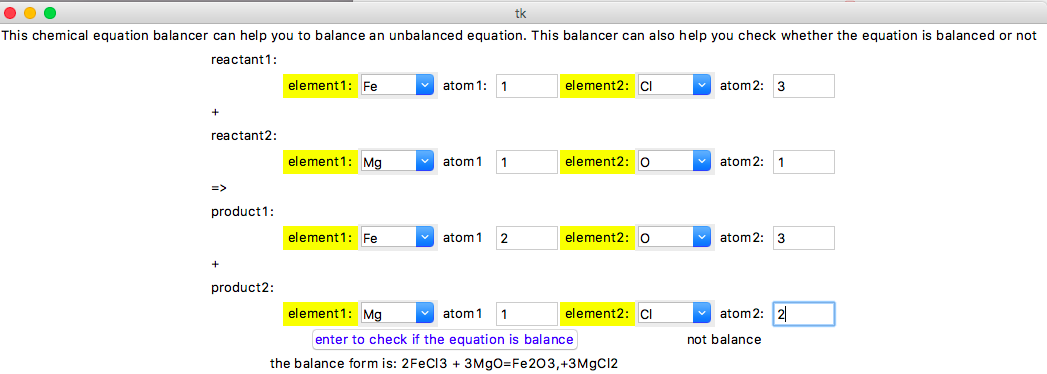
\includegraphics [width=\textwidth]{nonbalance}
 \caption{\label{ Figure 7:} non balance reaction}
 \end{center}
 \end{figure}

\subsection{Molecular Weight Calculation Test-id6}

The goal of this test is to get molecular weight for a reactant. Picture below shows molecular weight is printed for reactant " $Fe_2$$O_3$" as the test case id6 in \cite{SystemVnVPlan} and the result is identical. Test passed correctly and system responded as intended.

\begin{figure}[H]
 \begin{center}
 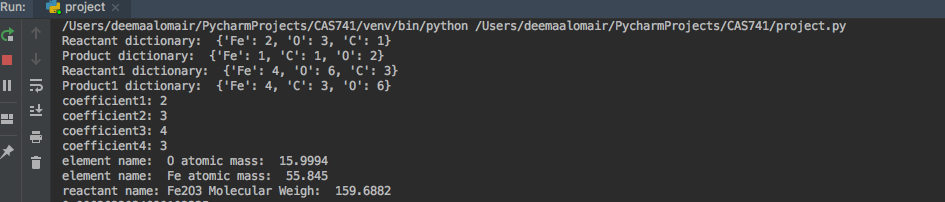
\includegraphics [width=\textwidth]{molecularweight}
 \caption{\label{ Figure 8:} molecular weight value}
 \end{center}
 \end{figure}

\subsection{Mole1 Calculation Test-id7}

The goal of this test is to get mole for reactant with known mass. we name this mole "Mole1". Picture below shows Mole1 value printed for reactant " $Fe_2$$O_3$" as the test case id7 in \cite{SystemVnVPlan} and the result is identical. Test passed correctly and system responded as intended.

\begin{figure}[H]
 \begin{center}
 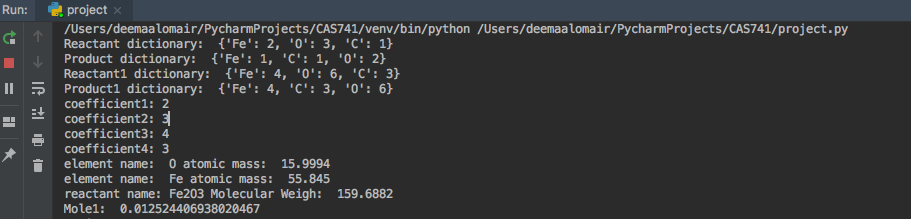
\includegraphics [width=\textwidth]{mole1}
 \caption{\label{ Figure 9:} Mole1 value}
 \end{center}
 \end{figure}

\subsection{Mole Ratio Calculation Test-id8}

The goal of this test is to get mole ratio between given reactants. Picture below shows Mole Ratio value for coefficient of reactant2/coefficient of reactant1 printed  as the test case id8 in \cite{SystemVnVPlan} and the result is identical. Test passed correctly and system responded as intended.

\begin{figure}[H]
 \begin{center}
 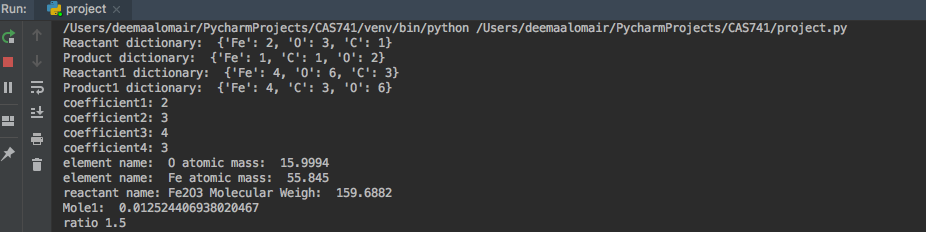
\includegraphics [width=\textwidth]{moleratio}
 \caption{\label{ Figure 10:} Mole Ratio value}
 \end{center}
 \end{figure}

\subsection{Mole2 Calculation Test-id9}

The goal of this test is to get mole for reactant with unknown mass. we name this mole "Mole2". Picture below shows Mole2 value printed as the test case id9 in \cite{SystemVnVPlan} and the result is identical. Test passed correctly and system responded as intended.

\begin{figure}[H]
 \begin{center}
 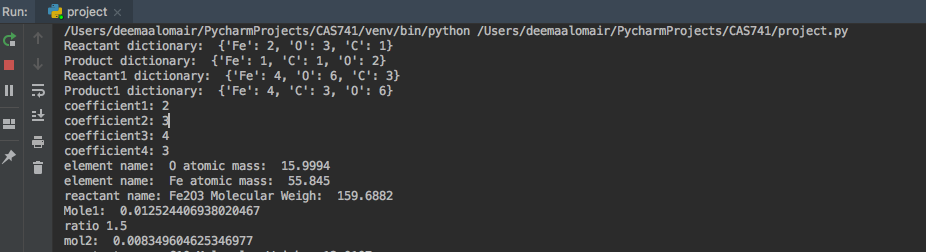
\includegraphics [width=\textwidth]{mole2}
 \caption{\label{ Figure 11:} Mole2 value}
 \end{center}
 \end{figure}
 
\subsection{Mass Calculation Test-id10}

The goal of this test is to get the final mass result for reactant with unknown mass. Picture below shows mass value printed as the test case id10 in \cite{SystemVnVPlan} and the result is identical. Test passed correctly and system responded as intended.

\begin{figure}[H]
 \begin{center}
 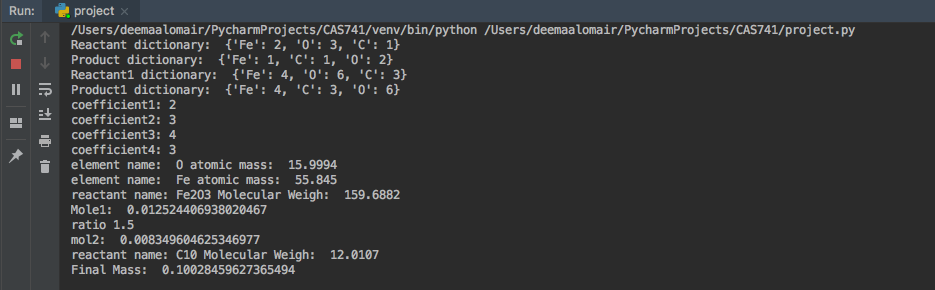
\includegraphics [width=\textwidth]{mass2}
 \caption{\label{ Figure 12:} final mass value}
 \end{center}
 \end{figure}

\section{Changes Due to Testing}

No changes are necessary to the first stage of implementation due to these test results.

\section{Automated Testing}

\begin{itemize}
\item coverage testing was preformed using coverage package without any error. blew picture shows coverage testing.
\end{itemize}

\begin{figure}[H]
 \begin{center}
 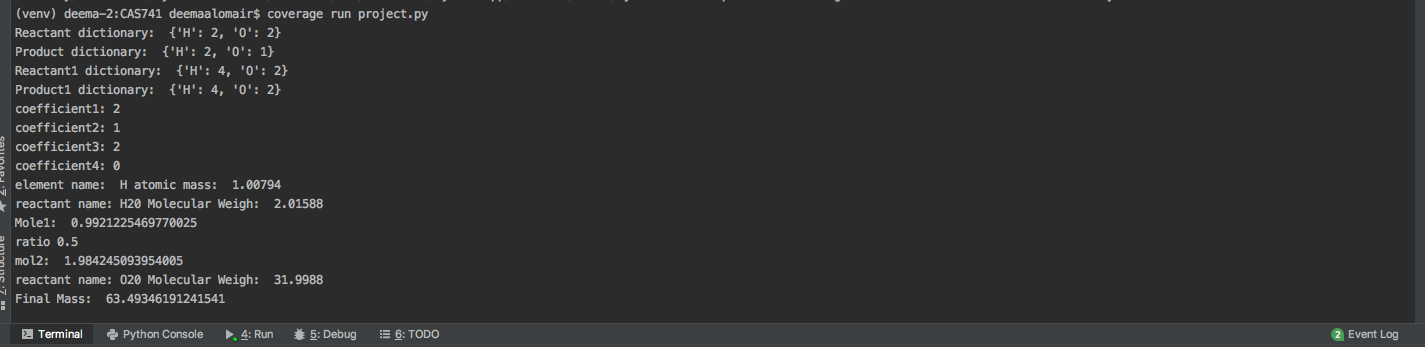
\includegraphics [width=\textwidth]{coverage}
 \caption{\label{ Figure 13:} coverage testing}
 \end{center}
 \end{figure}


\section{Trace to Requirements}\label{functional}

\begin{table}[h!]
\centering
\resizebox{\textwidth}{!}{\begin{tabular}{|c|c|c|c|c|c|c|c|c|c|c|}
\hline
  & id1 & id2 & id3 & id4 & id5 & id6 & id7 & id8 & id9 & id10  \\
\hline
R1(input)  & X& X& & & & & & & &   \\ \hline
R2(output)  & & & X& X& & & & & & \\ \hline
R3(calculation) & & & & & &X &X&X & X &  X \\ \hline
R4(VerifyInputOutput)  & X&X &X & X& & & & & &  \\ \hline
\hline
\end{tabular}}
\caption{Traceability Matrix Showing the Connections Between unit test cases and functional requirements}
\label{Table:R_trace}
\end{table}

\begin{table}[h!]
\centering
\begin{tabular}{|c|c|c|}
\hline
  & id11 & id12   \\
\hline
NF1  & & X \\ \hline
NF2  & X& \\ \hline
\hline
\end{tabular}
\caption{Traceability Matrix Showing the Connections Between unit test cases and Nonfunctional requirements}
\label{Table:R_trace1}
\end{table}

\section{Trace to Modules}	
	
A complete description of modules is found in the MG \cite{Designdocument}.
\begin{table}[h!]
\centering
\resizebox{\textwidth}{!}{\begin{tabular}{|c|c|c|c|c|c|c|c|c|c|c|}
\hline
  & id1 & id2 & id3 & id4 & id5 & id6 & id7 & id8 & id9 & id10  \\
\hline
Input Module  & X& X& & & & & & & &   \\ \hline
Atomic Mass Module  & & & & & & X& & & & \\ \hline
Balancing Chemical Reaction Module & & & X& & X& & & &  &   \\ \hline
Mass Calculation Module  & & & & & & X&X &X & X& X  \\ \hline
GUI Module  & & &X & X& & & & & &  \\ \hline
\hline
\end{tabular}}
\caption{Traceability Matrix Showing the Connections Between Modules and Test Cases}
\label{Table:R_trace2}
\end{table}

\section{Code Coverage Metrics}

coverage test was done for the whole system and covers all functional requirements. It covers test cases from id1 to id10. 

\newpage
\bibliographystyle{unsrt}

\bibliography{../../refs/References}

\end{document}
